%!TEX root = ../tesi.tex

\chapter{Il Progetto SF-Remote-Connection}
\label{ch:sfremoteconnection}

Vengono ora presentati i moduli software realizzati nel corso del progetto di tesi.
Per meglio comprendere gli aspetti di sviluppo legati al progetto \`e importante tener conto degli obbiettivi esposti al paragrafo \ref{sec:obbiettivo} e della descrizione dei meccanismi di gestione dati interni del framework, descritti nel capitolo \ref{ch:gestionedati}.

Nella sezione \ref{sec:moduli} del capitolo viene fornita innanzitutto una suddivisione e una descrizione dei moduli, nella sezione \ref{sec:dataset_sost} viene descritto il meccanismo dei Dataset sostitutivi e nella \ref{sec:rete} l'infrastruttura di rete e il protocollo di comunicazione.

L'obiettivo principale ha riguardato la produzione di librerie e tool per lo sviluppo di applicazioni, focalizzandosi sull'estendibilit\`a e il riutilizzo del codice. Non a caso sono infatti presenti alcuni riferimenti di appendice ad alcuni design pattern particolarmente significativi nella produzione di questo tipo di software e che sono utilizzati sia dal framework che dai moduli stessi.

Per il processo di sviluppo \`e stata di fondamentale importanza la produzione parallela di una serie di test, presentati nel capitolo \ref{ch:testerisultati}. Infatti la progettazione e la realizzazione dei moduli e dei meccanismi presentati in questo capitolo non \`e stata svolta in maniera distinta, ma si \`e trattato di un processo iterativo in cui i test hanno svolto pi\`u di una volta un ruolo di guida nel refactoring del codice.

Si rimanda all'appendice \ref{a:notesoftware} per informazioni sul codice sorgente relativo al progetto e per informazioni sulle versioni delle librerie utilizzate.

\section{Moduli} 
\label{sec:moduli}
La libreria di classi realizzata pu\`o essere suddivisa in quattro macro-moduli suddivisi in base alle finalit\`a e alle funzionalit\`a.
Di seguito viene data una descrizione degli stessi in questo ordine:
\begin{enumerate}
	\item \textbf{Base Communication}
	\item \textbf{RemoteDataCenter Tool}
	\item \textbf{Client}
	\item \textbf{Server}
\end{enumerate}

% TODO: 
%	inserire un'immagine di come i moduli funzionino su vari livelli
%	verificare i nomi e le appartenenze dei package

\subsection{Base Communication}
\label{sub:basecommodule}
Questo modulo riunisce le classi che consentono la creazione e la gestione di connessioni TCP/IP tra applicazioni client/server. Ne fa parte anche la classe di utilit\`a \texttt{GenericCommunicator} che oltre a consentire la gestione della connessione assegnatagli la utilizza per fornire funzionalit\`a di lettura e scrittura di messaggi testuali attraverso il canale aperto.

Di grande importanza per questo modulo sono anche la classe \texttt{CommunicationProtocol} e l'interfaccia \texttt{ICommunicationProtocolTask} che, come vedremo nei casi di \textbf{Client} e \textbf{Server}, possono essere utilizzate da moduli esterni che sfruttano il design pattern \textit{State}\footnote{Il pattern \textit{State} viene descritto al paragrafo \ref{sub:state}} per gestire il protocollo di comunicazione attraverso una macchina a stati.

Il modulo \`e composto dai package \texttt{sfrc.base.communication} e \\\texttt{sfrc.base.communication.sfutil}.

\subsection{RemoteDataCenter Tool}
\label{sub:remotedatacentertoolmodule}

\begin{figure}[t]
\begin{center}
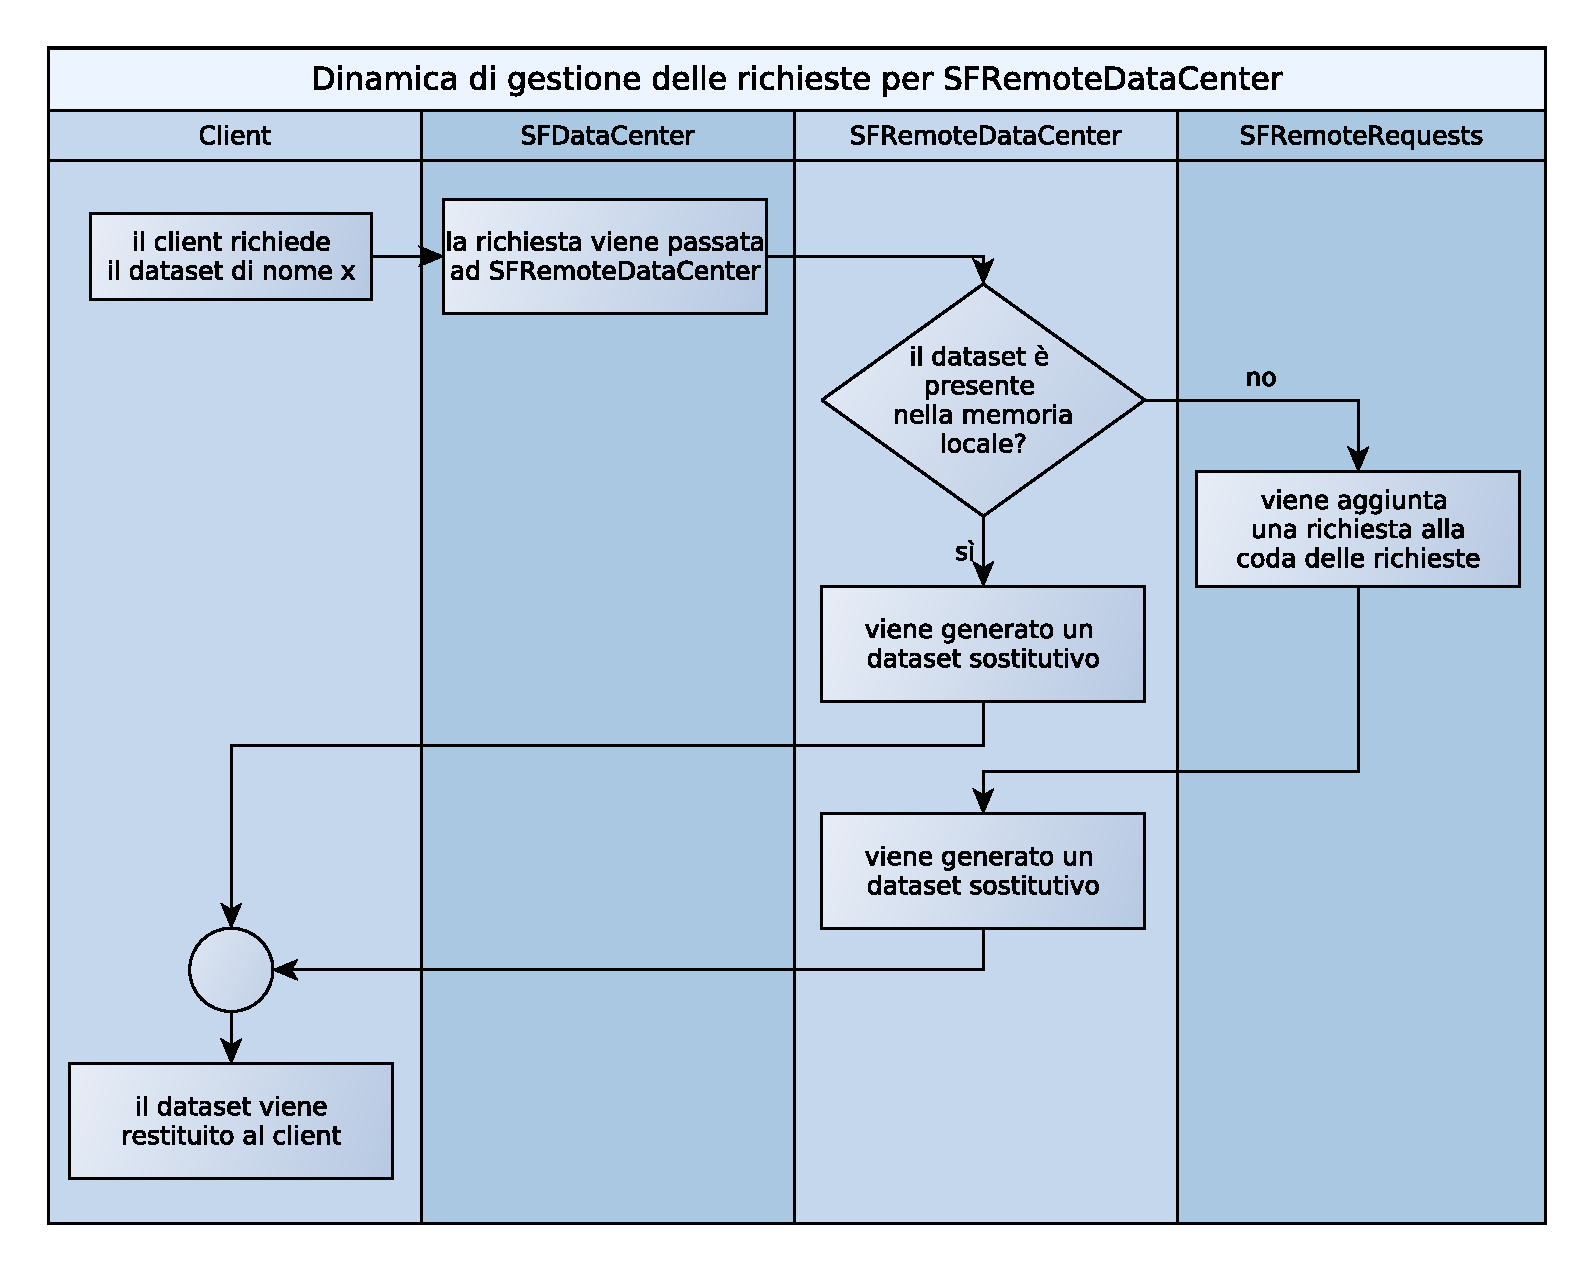
\includegraphics[width=\textwidth]{Immagini/DinamicaSFRemoteDataCenter}
\caption[Sequenza di eventi di una richiesta a SFRemoteDataCenter.]{Lo schema mostra la sequenza di eventi dovuti ad una richiesta a SFDataCenter che utilizza un SFRemoteDataCenter come implementazione interna.\label{f:dinamicasfremotedatacenter}} 
\end{center} 
\end{figure}

Questo modulo raggruppa una serie di classi pensate per estendere il framework e per essere utilizzate all'interno di una applicazione client.
La funzione principale consiste nel fornire uno strato di comunicazione tra l'astrazione del reperimento dati fornita dal framework e il meccanismo di effettivo reperimento dei dati.

La classe chiave del modulo \`e \texttt{SFRemoteDataCenter} la quale \`e una classe di implementazione utilizzabile nel \textit{Bridge} realizzato da \texttt{SFDataCenter}\footnote{Per la classe \texttt{SFDataCenter} si rimanda al paragrafo \ref{sub:sfdatacenter} mentre per il pattern \textit{Bridge} al paragrafo \ref{sub:bridge}.}.
Dallo schema in figura \ref{f:dinamicasfremotedatacenter} osserviamo che le richieste di Dataset effettuate al DataCenter vengono passate a questa classe che le esamina verificando che il dato richiesto sia presente nella libreria dell'applicazione. Se il Dataset non \`e presente viene generata una richiesta e aggiunta ad un buffer di richieste di nome \texttt{SFRemoteDataCenterRequests}, mentre al richiedente viene restituito un Dataset sostitutivo temporaneo scelto opportunamente. Il buffer, che supporta la sincronizzazione, pu\`o contemporaneamente essere utilizzato da un modulo esterno in grado di effettuare l'effettivo reperimento dei dati.
Il meccanismo dei Dataset sostitutivi viene descritto esaustivamente nella sezione \ref{sec:dataset_sost}.

% TODO: decidere se i 2 package aggiuntivi andrebbero inseriti nel modulo
Il modulo \`e composto dai package \texttt{shadow.system.data.remote.wip}, \texttt{shadow.system.data.object.wip} e \texttt{shadow.renderer.viewer.wip}.

\subsection{Client}
\label{sub:clientmodule}
Questo modulo raggruppa delle componenti generiche che possono essere utilizzate all'interno di una qualsiasi applicazione client e che servono ad implementare l'effettivo reperimento dei dati. 
Esso si pone al di sotto del modulo \textbf{RemoteDataCenter Tool} ed utilizza il modulo \textbf{Base Communication} per la gestione del canale di comunicazione e la sua implementazione \`e pensata per il multi-threading.
Il meccanismo messo a disposizione \`e mostrato nella figura \ref{f:dinamicaclient}, dove un thread \texttt{RemoteDataCenterRequestsCreationTask} viene risvegliato periodicamente e controlla che non vi siano richieste pendenti nel buffer delle richieste. Se il buffer non \`e vuoto viene allocano un nuovo thread di tipo \texttt{RemoteDataCenterRequestTask} e mentre il precedente viene nuovamente sospeso questo effettua le richieste al server. Quando il secondo thread termina la comunicazione chiede al buffer di generare un update a tutti i client che avevano richiesto i dati reperiti e successivamente si chiude.


\begin{figure}
\begin{center}
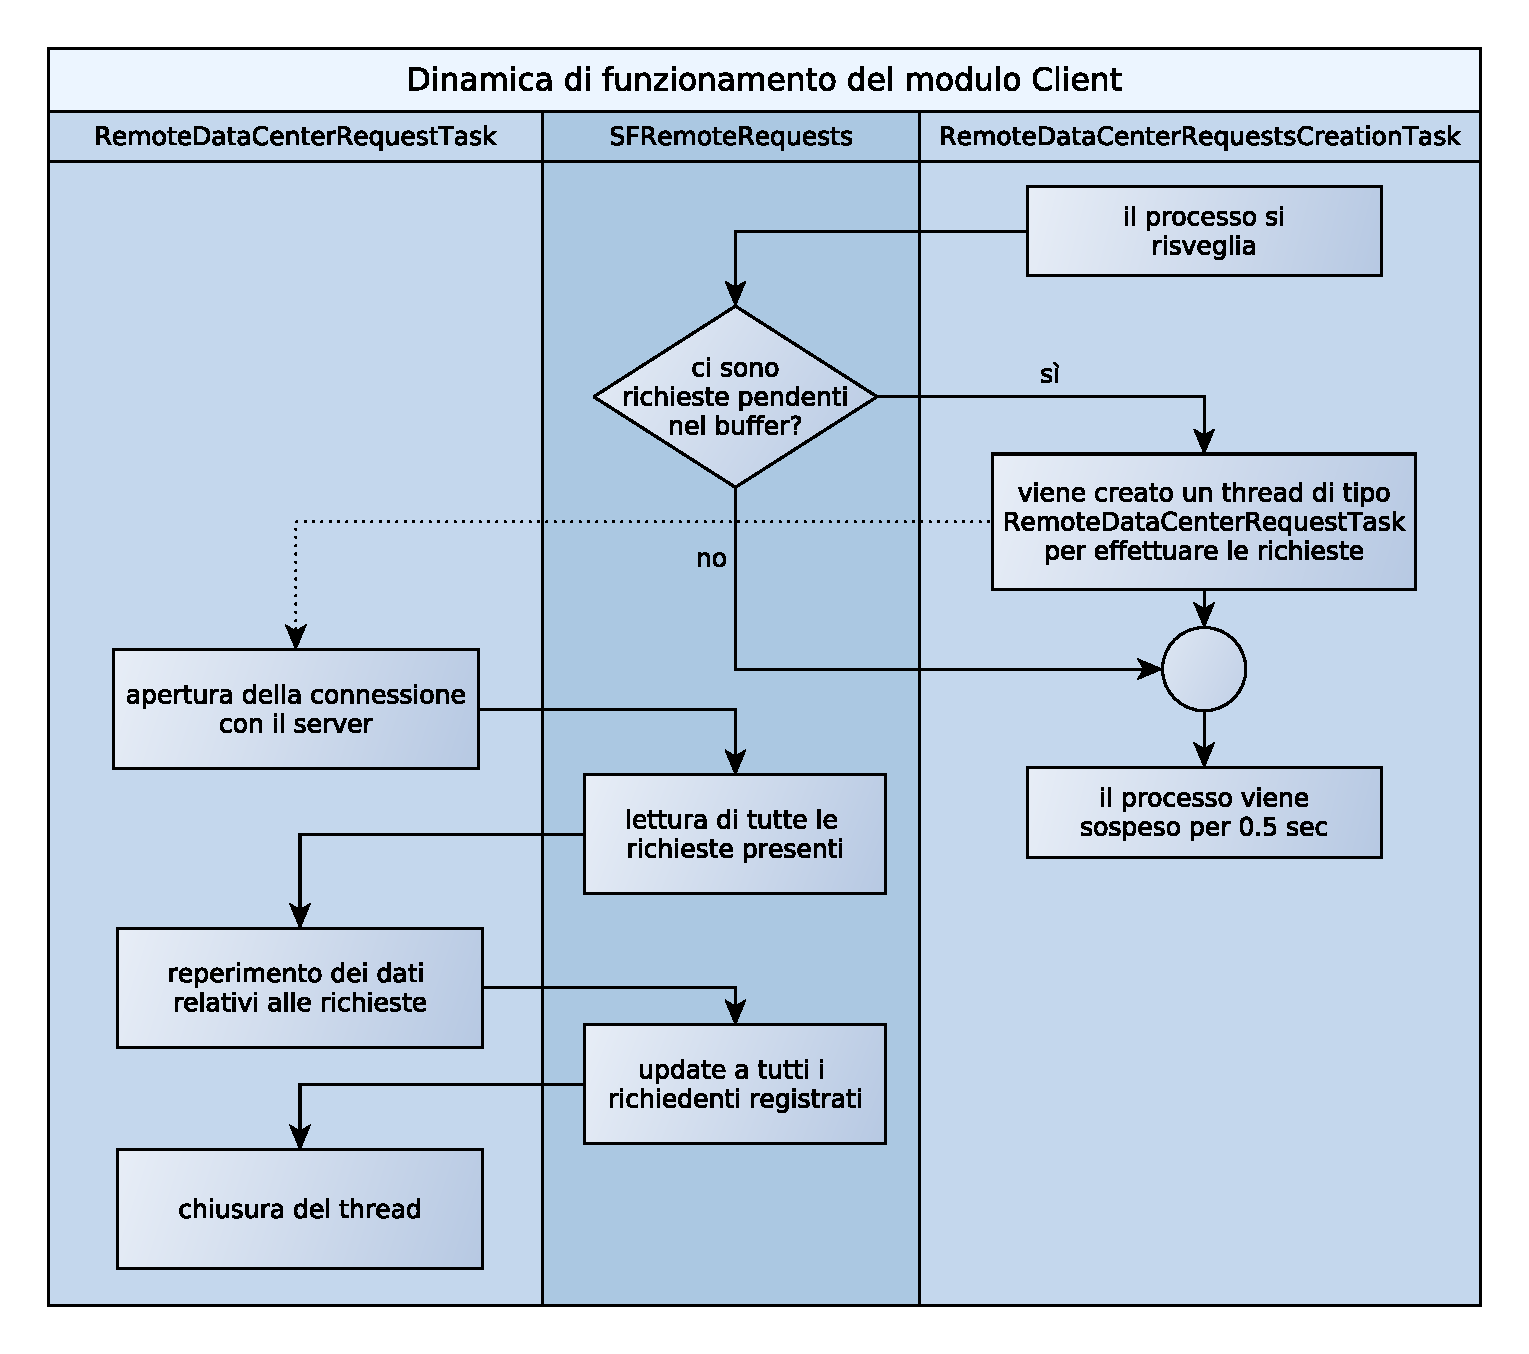
\includegraphics[width=\textwidth]{Immagini/DinamicaClient}
\caption[Dinamica del modulo client.]{Nello schema presentato viene messa in evidenza la sostanziale indipendenza dei thread \texttt{RemoteDataCenterRequestsCreationTask} e \texttt{RemoteDataCenterRequestTask}, infatti escludendo la generazione dei thread del secondo tipo da parte del primo, non vi sono comunicazioni dirette tra essi.\label{f:dinamicaclient}} 
\end{center} 
\end{figure}


Il package che compone questo modulo \`e \texttt{sfrc.application.client}.

\subsection{Server}
\label{sub:servermodule}
Similmente a quello per le componenti client, in questo modulo vengono raggruppate delle componenti generiche utili alla realizzazione di una applicazione server. Queste componenti fungono da tramite tra l'applicazione e il modulo di \textbf{Base Communication} grazie al quale realizzano l'effettivo trasferimento dei Dataset verso il client connesso.
L'implementazione \`e pensata per il funzionamento multi-thread in parallelo con l'applicazione principale che pu\`o cos{\`\i} gestire pi\`u client connessi contemporaneamente ed eseguire altre operazioni.
Vengono fornite infine anche delle interfacce utili per effettuare l'inizializzazione dei dati e per configurare il protocollo di comunicazione.

Il modulo \`e composto dal package \texttt{sfrc.application.server}

\section{Dataset sostitutivi}
\label{sec:dataset_sost}
Per evitare che, in seguito alla richiesta di un Dataset non presente nella libreria locale di un'applicazione, i moduli richiedenti rimanessero in attesa dei dati bloccando di fatto l'esecuzione, \`e stato realizzato un meccanismo che sostituisce i dati richiesti con dei Dataset alternativi, gi\`a presenti nella memoria del client. Al successivo arrivo dei dati reali viene effettuato un update tramite i meccanismi di sincronizzazione offerti dal framework.

\begin{figure}
\begin{center}
\includegraphics[width=\textwidth]{Immagini/sequenzaDatiSost}
\caption{Diagramma di sequenza del meccanismo a Dataset sostitutivi.\label{f:seqsost}} 
\end{center} 
\end{figure}

Il diagramma di sequenza in figura \ref{f:seqsost} mostra la dinamica temporale di funzionamento del sistema nel caso in cui l'applicazione richieda un Dataset non ancora presente in memoria: l'applicazione effettua la richiesta ad \texttt{SFDataCenter} passandone il nome e la callback necessaria per restituire il dato.
Questi vengono poi passati ad \texttt{SFRemoteDataCenter} che, una volta appurata l'assenza del dato in memoria, registra alla coda delle richieste \texttt{SFRemoteDataCenterRequests} prima la callback e poi la richiesta stessa. L'\texttt{SFRemoteDataCenter} genera successivamente un Dataset sostitutivo (TmpDataset) che viene usato come parametro quando viene chiamata la callback \texttt{listener.onDatasetAvailable(TmpDataset)}.
Quando il modulo di reperimento dei dati riceve il Dataset reale lo notifica alla coda attraverso il metodo \texttt{onRequestUpdate(...)}.

\texttt{SFRemoteDataCenterRequests} prende in carico il compito di effettuare l'update, richiamando tutte le callback registrate e associate al dato ricevuto.

Il passaggio critico dell'aggiornamento dei dati, soprattutto quelli grafici, viene effettuato sfruttando il meccanismo dell'Updater mostrato nella sezione \ref{sec:dati grafici}.

Sfruttando il fatto di non bloccare l'esecuzione in attesa dei dati, l'utilizzo dei Dataset sostitutivi consente la visualizzazione di una scena in cui i modelli oggetto della simulazione sono temporaneamente rimpiazzati da dei segnaposto, ma in cui \`e gi\`a possibile navigare all'interno e avviare l'interazione con l'ambiente circostante. La scelta dei dati sostitutivi da parte di \texttt{SFRemoteDataCenter} deve essere effettuata in maniera appropriata a seconda dell'oggetto che si deve rimpiazzare, ma per permettere il funzionamento di questo automatismo si \`e resa necessaria la realizzazione di un nuovo tipo di Dataset, l'SFDatasetReplacement, e di una libreria di Dataset sostitutivi.

Utilizzato all'interno di una ObjectsLibrary un DatasetReplacement permette di realizzare una lista di sostituzione che associa il nome di un Dataset ``Alfa'' richiesto, a quello di un Dataset sostitutivo di default ``Beta'' e ad un timestamp.

Se l'associazione tra nomi viene usata per una ricerca diretta del dato sostitutivo da utilizzare, il timestamp \`e stato introdotto per lo sviluppo futuro di logiche di aggiornamento della lista di sostituzione, attraverso un confronto dei timestamp locali con quelli remoti. Sul server si possono cos{\`\i} inserire meccaniche di modifica ed espansione dell'ambiente simulato centralizzate ed automatizzate che non richiedano all'utente di bloccare la fruizione dei contenuti nell'attesa del download degli aggiornamenti.

L'utilizzo di questo automatismo richiede necessariamente una fase di inizializzazione in cui viene fatto il download o il caricamento da disco locale della lista di sostituzione e della libreria dei Dataset di default. Avendo la possibilit\`a di integrare il protocollo di comunicazione estendendo le due librerie durante l'esecuzione, \`e possibile mantenere la loro dimensione iniziale contenuta.

La libreria di Dataset sostitutivi viene descritta in maggiore dettaglio nella sezione \ref{sec:correlate}.

\section{Infrastruttura di rete} 
\label{sec:rete}
Date le specifiche iniziali esposte nel capitolo \ref{ch:introduzione}, una parte fondamentale del progetto \`e stata decidere quale infrastruttura per la comunicazione di rete sfruttare per poter utilizzare e testare il modulo \textbf{RemoteDataCenter Tool}, che si occupa della gestione delle richieste di Dataset.

Se da lato client \`e ovvia la necessit\`a di sviluppare uno strato dell'applicazione che si occupa della comunicazione di rete, da lato server si sono presentate diverse possibilit\`a: 

\begin{enumerate}
	\item  utilizzare un file server che permettesse semplicemente di accedere ai file contenenti i dati tramite la rete;
	\item  utilizzare un application server java, come Tomcat o Glassfish, a cui un'applicazione client potesse connettersi e che attraverso l'esecuzione di servlet realizzasse il trasferimento dei dati da server a client;
	\item  utilizzare un'applicazione server ad-hoc appositamente sviluppata;
\end{enumerate}

La prima soluzione \`e probabilmente la pi\`u semplice, ma la meno flessibile poich\'e consente solo un accesso diretto ai file di descrizione dei dati senza alcuna possibilit\`a di un'elaborazione lato server e spostando tutto il peso computazionale di un'eventuale interazione tra client direttamente su quest'ultimi.

La seconda soluzione offre pi\`u possibilit\`a e flessibilit\`a rispetto alla prima: l'utilizzo di un application server java mette a disposizione una piattaforma che consente una pre-elaborazione dei dati lato server e possiede direttamente una serie di componenti per la gestione di compiti complessi legati alle sessioni degli utenti, come ad esempio l'autenticazione e la sicurezza. 
Nonostante i pregi, questo tipo di soluzione presenta lati negativi: gli application server generici non sono sviluppati per questo tipo di applicazioni e non \`e garantita una flessibilit\`a sufficiente per cui all'aumentare della complessit\`a del progetto, e delle sue esigenze non sia necessario abbandonare l'architettura. 

La terza soluzione \`e sicuramente la pi\`u flessibile ed estendibile poich\'e consente di modificare direttamente il server per adattarsi alle esigenze dell'applicazione. Lo svantaggio \`e la necessit\`a di dover implementare da zero tutte quelle funzionalit\`a non solo di comunicazione, ma anche di autenticazione o di sicurezza che una soluzione gi\`a pronta potrebbe possedere nativamente.

Nella scelta tra le tre soluzioni hanno condizionato la volont\`a di realizzare un'architettura funzionante con la scrittura di meno codice possibile e quella di mantenere una bassa complessit\`a iniziale che non penalizzasse un'estensione futura delle funzionalit\`a. In quest'ottica la prima soluzione \`e stata la prima ad essere scartata, perch\'e sebbene garantisse un tempo di messa in opera molto basso, non consente un'estensione di funzionalit\`a. 

La scelta finale \`e ricaduta sulla terza soluzione che pur costringendo a rinunciare alle funzionalit\`a avanzate della seconda, elimina difficolt\`a e tempistiche di una installazione e configurazione dell'application server. Inoltre, limitando inizialmente lo sviluppo alle funzionalit\`a di base, \`e possibile ridurre la complessit\`a del codice ad un livello non pi\`u elevato rispetto alla seconda soluzione.

\subsection{Protocollo di comunicazione}
\label{sub:comprotocol}
Una volta stabilito di utilizzare un server sviluppato appositamente \`e stato necessario stabilire le modalit\`a di comunicazione tra client e server. 

La comunicazione tra le applicazioni viene effettuata attraverso un protocollo basato su messaggi testuali che si colloca idealmente a livello di Sessione nel modello ISO/OSI \cite{book:computernetworking} mentre a livello inferiore viene utilizzato il protocollo TCP/IP.
L'utilizzo del TCP, in quanto protocollo confermato, \`e giustificato in quanto garantisce la ricezione dei messaggi di comunicazione. Poich\'e questi sono principalmente dedicati allo scambio di dati grafici, la garanzia di ricezione e d'integrit\`a risultano prioritari rispetto alle prestazioni.

I messaggi di comunicazione finora previsti sono strutturati secondo la seguente forma:
\begin{verbatim}
     etichetta_messaggio[:dati:opzionali:...]
\end{verbatim}
in cui \texttt{etichetta\_messaggio} identifica il tipo di messaggio, mentre i dati opzionali dipendono dal messaggio stesso e sono divisi dall'etichetta e tra loro dal carattere `` : ''.

\begin{figure}[t]
\begin{center}
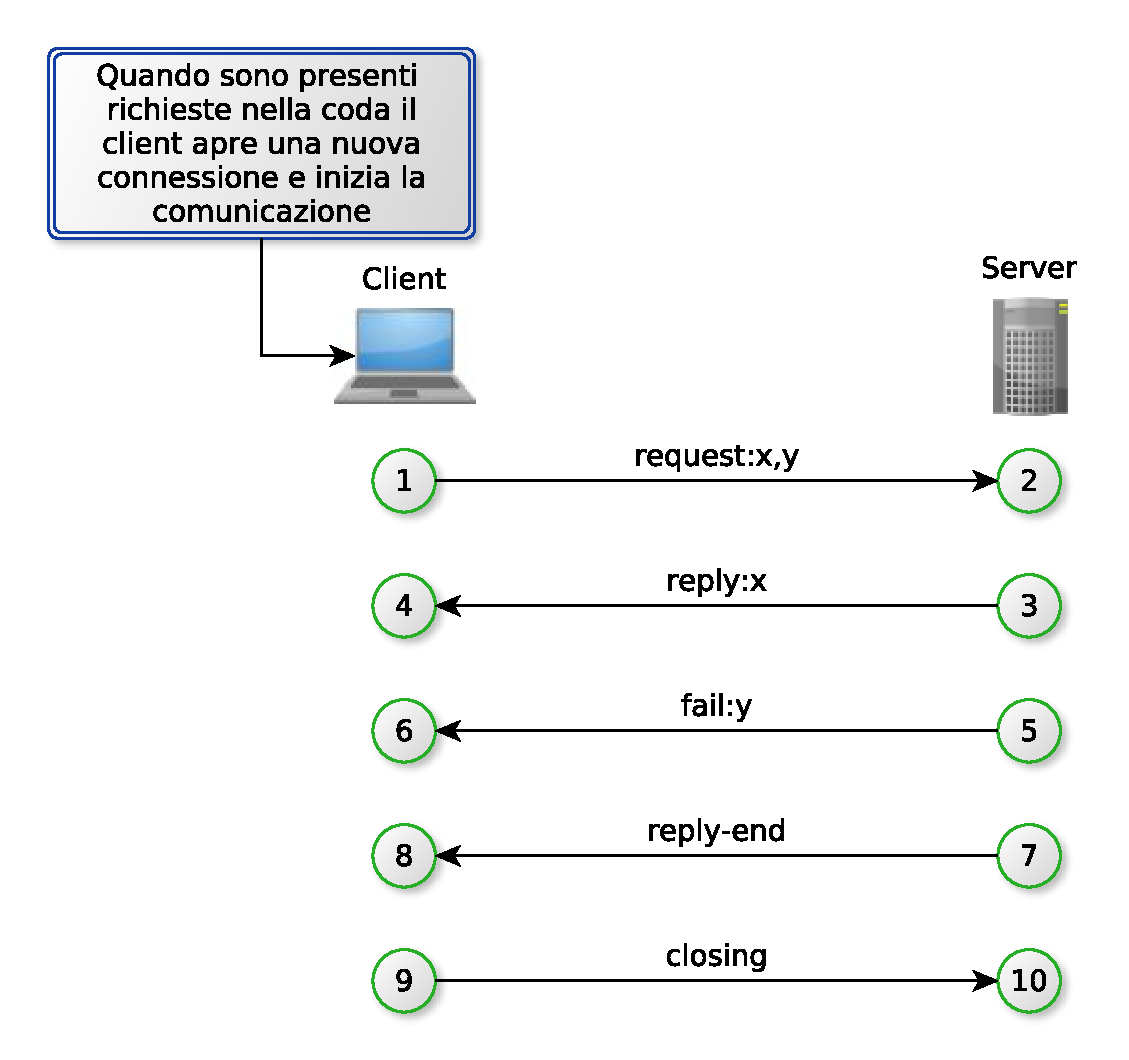
\includegraphics[width=10cm]{Immagini/InterazioniClientServer}
\caption{Esempio dello schema di interazione tra client e server.\label{f:clientserverinteraction}} 
\end{center} 
\end{figure}

I messaggi sono utilizzati all'interno di un preciso schema di interazione tra client e server di cui possiamo vedere un esempio nella figura \ref{f:clientserverinteraction}, in cui la numerazione dei nodi rappresenta la sequenza temporale dello scambio di messaggi. 
Lo schema illustra che, quando la coda delle richieste non \`e vuota, il client apre una connessione con il server ed invia un messaggio di tipo \textbf{request} in cui sono elencati i nomi dei Dataset richiesti. Il server a questo punto genera una sequenza di risposte attraverso cui invia, se possibile, i dati richiesti. Al termine della sequenza invia un messaggio di tipo \textbf{reply-end} a cui il client risponde con un messaggio \textbf{closing} per terminare la connessione. La gestione della comunicazione e dello schema di interazione viene effettuata tramite una macchina a stati specifica, una per il client e una per il server, ognuna delle quali si occupa di leggere ed effettuare l'analisi logico-sintattica dei messaggi generando le eventuali risposte o semplicemente modificando lo stato interno della macchina stessa.

Usare messaggi testuali per la comunicazione consente di semplificarne la gestione e rende possibile espandere il linguaggio semplicemente utilizzando nuove etichette, tuttavia l'implementazione della macchina a stati deve essere strutturata in modo da garantire l'espandibilit\`a.

Per questo motivo \`e stato preso come modello il pattern \textit{State}, descritto al paragrafo \ref{sub:state}, e la logica di ogni stato \`e stata incapsulata in un oggetto differente. Questo consente di espandere la macchina a stati semplicemente definendo nuovi oggetti separando il codice della logica di gestione di ogni stato da quello degli altri.

\begin{figure}
\begin{center}
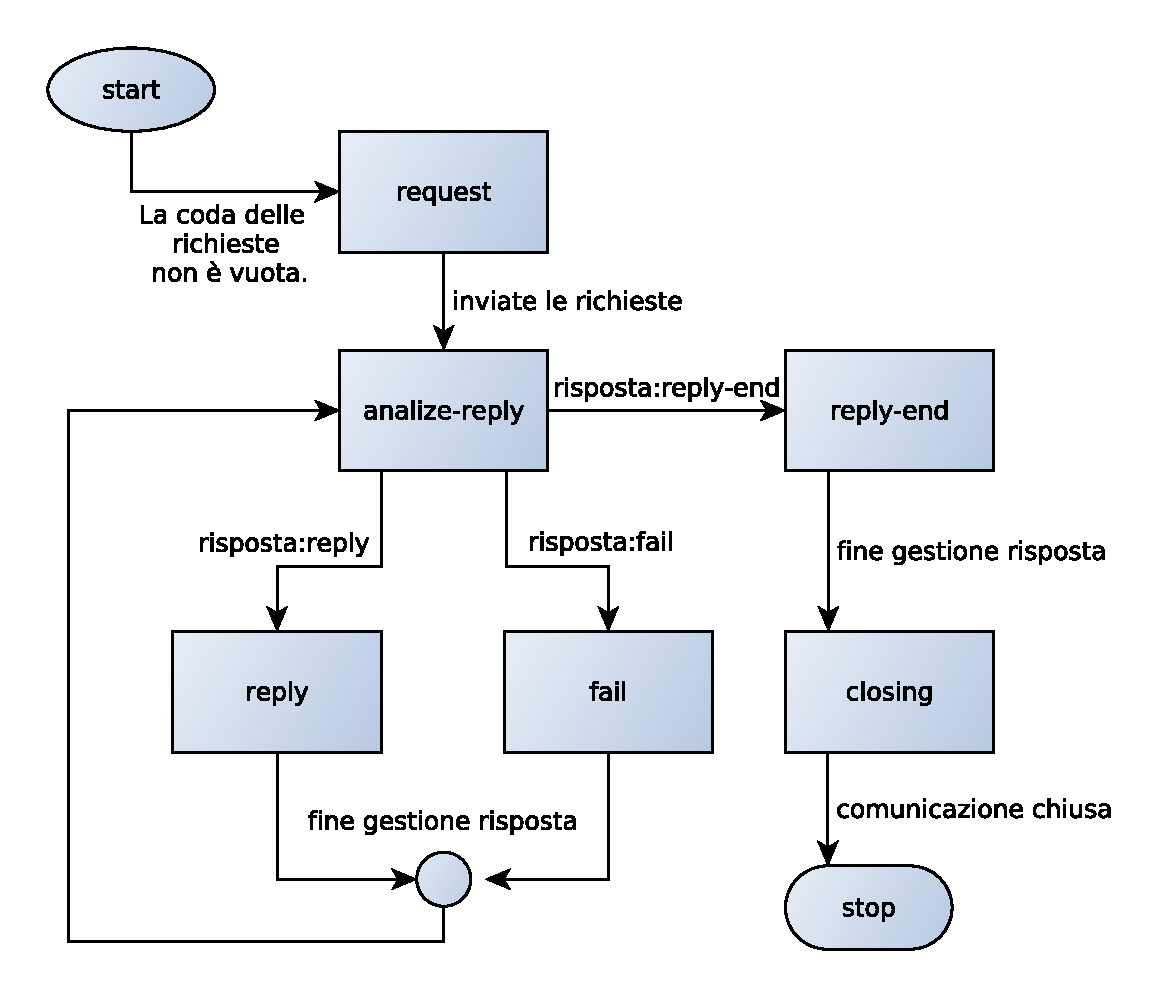
\includegraphics[width=11cm]{Immagini/StateMachineClient}
\caption{Diagramma a stati del client per la gestione delle richieste.\label{f:stateclient}} 
\end{center} 
\end{figure}

L'immagine in figura \ref{f:stateclient} mostra lo schema a blocchi della macchina a stati attualmente implementata nel modulo client per la gestione del protocollo di comunicazione. Lo stato iniziale dello schema \`e \textbf{request} ed \`e innescato dalla presenza di richieste nella coda. In questo stato il processo che gestisce la comunicazione invia le richieste al server e successivamente passa allo stato \textbf{analize-reply} in attesa di riceve le risposte.
Quando viene ricevuto il messaggio di risposta, viene estratta l'informazione sul tipo di messaggio determinando lo stato successivo della macchina. Se ad esempio la risposta \`e un messaggio di tipo \texttt{reply:nomedataset} lo stato successivo sar\`a quello corrispondente alla gestione di quel tipo di messaggio. Gli stati \textbf{reply} e \textbf{fail} si occupano di gestire il tipo di messaggio corrispondente e al termine della loro esecuzione la macchina torna nello stato di \textbf{analize-reply} in attesa di altre risposte.
All'arrivo del messaggio di fine risposte lo schema passa allo stato corrispondente di \textbf{reply-end} e poi a quello di \textbf{closing} dove chiede al server di chiudere la connessione. 

\begin{figure}
\begin{center}
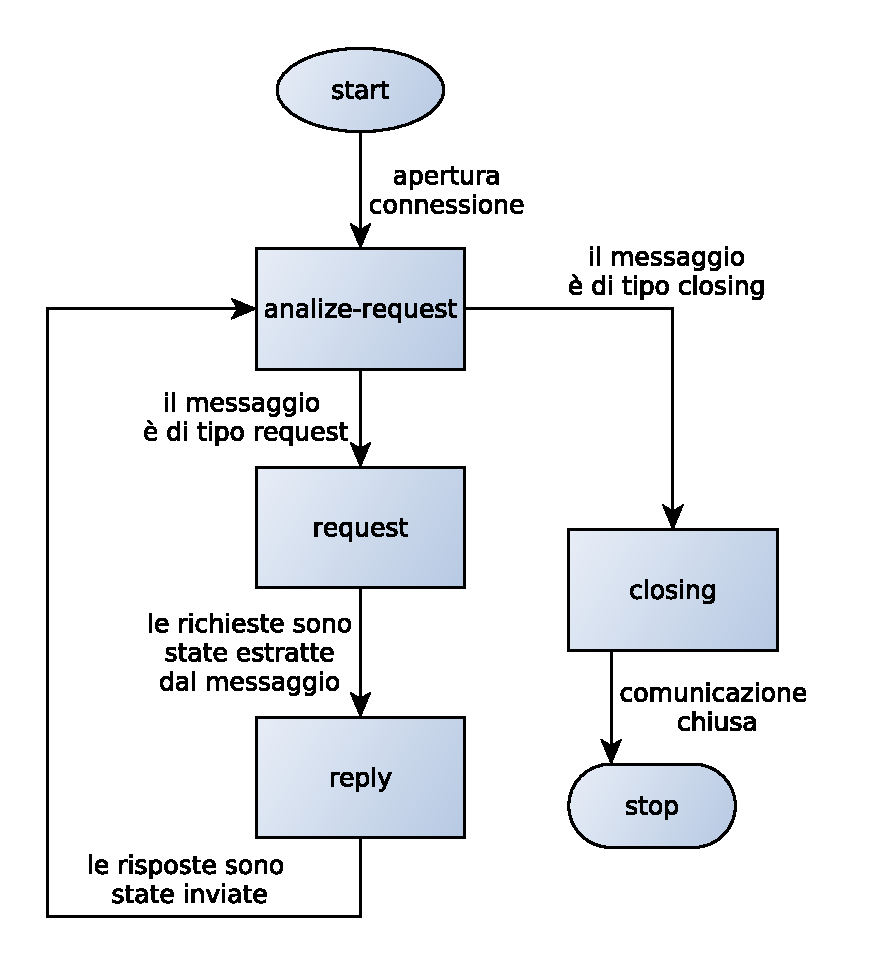
\includegraphics[width=10cm]{Immagini/StateMachineServer}
\caption{Diagramma a stati del server per la gestione delle richieste.\label{f:stateserver}} 
\end{center} 
\end{figure}

La figura \ref{f:stateserver} rappresenta invece lo schema implementato nel modulo server. All'apertura di una connessione il server entra nello stato \textbf{analize-request} dove rimane in attesa di messaggi di richiesta da parte del client. Alla ricezione di un messaggio di questo tipo, passa in uno stato \textbf{request} dove estrae dal messaggio i nomi di tutti i Dataset richiesti. Successivamente entra nello stato \textbf{reply} dove uno ad uno vengono inviati i dati di ogni Dataset richiesto per poi inviare un messaggio \texttt{reply-end} al termine della sequenza. Ritornato nello stato \textbf{analize-request} il server \`e in attesa di ulteriori richieste o di un messaggio di \texttt{closing} per entrare nello stato corrispondente dove viene terminata la comunicazione.

Le strutture delle macchine a stati di client e server non sono state definite per l'efficienza, ma per consentire la verifica dei meccanismi di livello pi\`u alto in differenti condizioni.

%I messaggi attualmente implementati sono:





% \section{I Package java} 
% \label{sec:sfrc_packages}
% La classi che compongono il progetto sono suddivise in una serie di package. % TODO: decidere se la prossima frase va bene
% Alcuni di questi sono pensati per rappresentare una possibile estensione a quelli forniti dal framework stesso e ne riproducono la struttura e le convenzioni sui nomi, gli altri sono librerie che affiancano il framework nella costruzione dell'applicazione.

